\section{Experiments}

\begin{figure}
    \centering
    \begin{subfigure}[b]{0.32\textwidth}
        \centering
        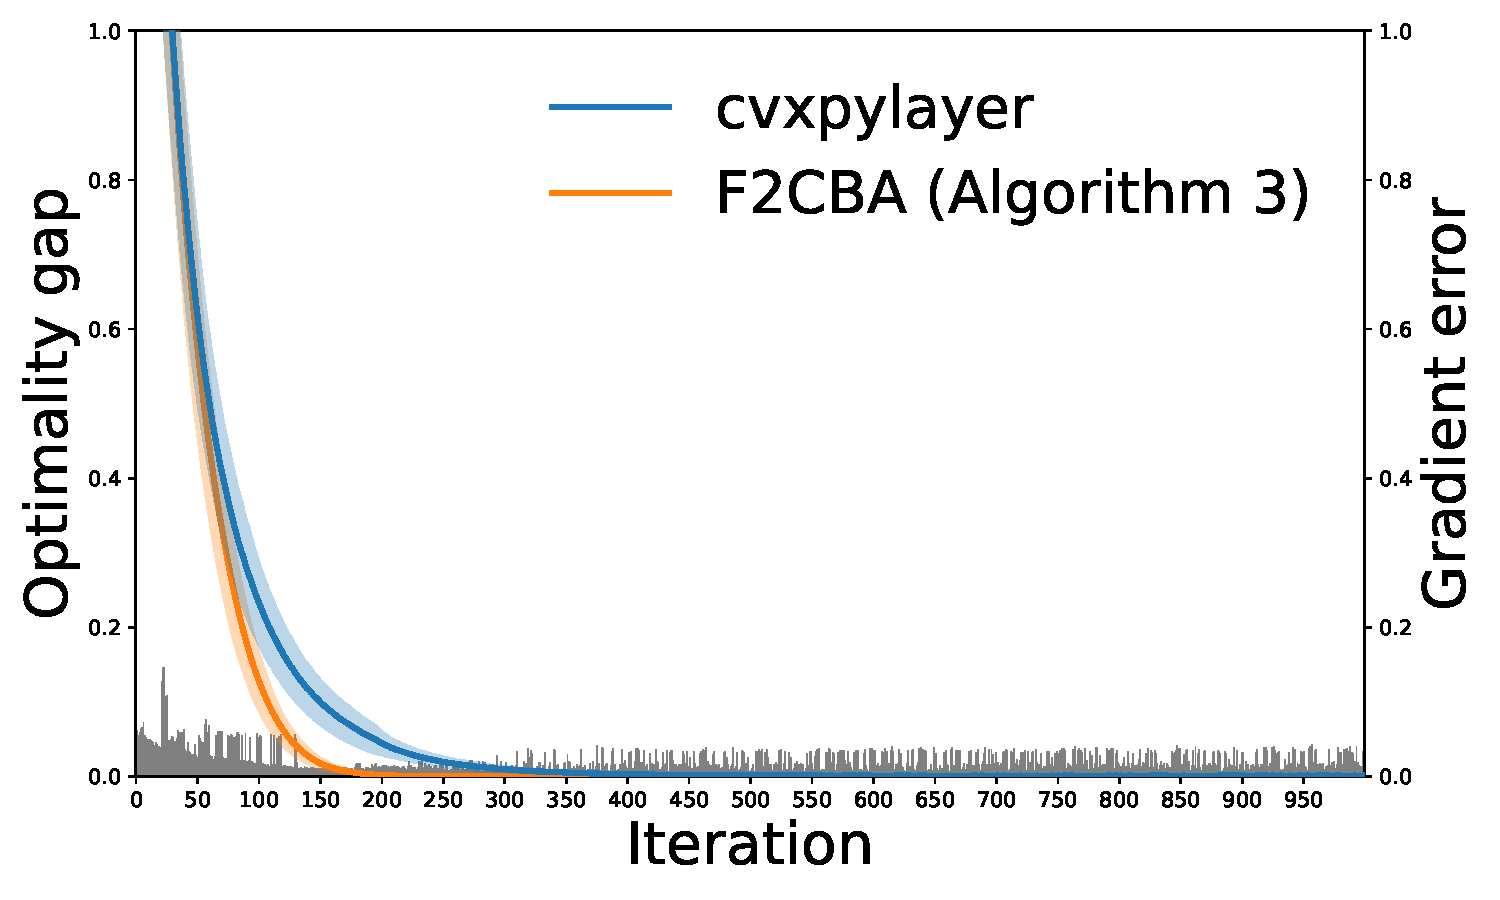
\includegraphics[width=\textwidth]{src/figures/ydim200_loss.pdf}
        \caption{Convergence comparison and gradient error plot.}
        \label{fig:convergence-comparison}
    \end{subfigure}
    \hfill
    \begin{subfigure}[b]{0.32\textwidth}
        \centering
        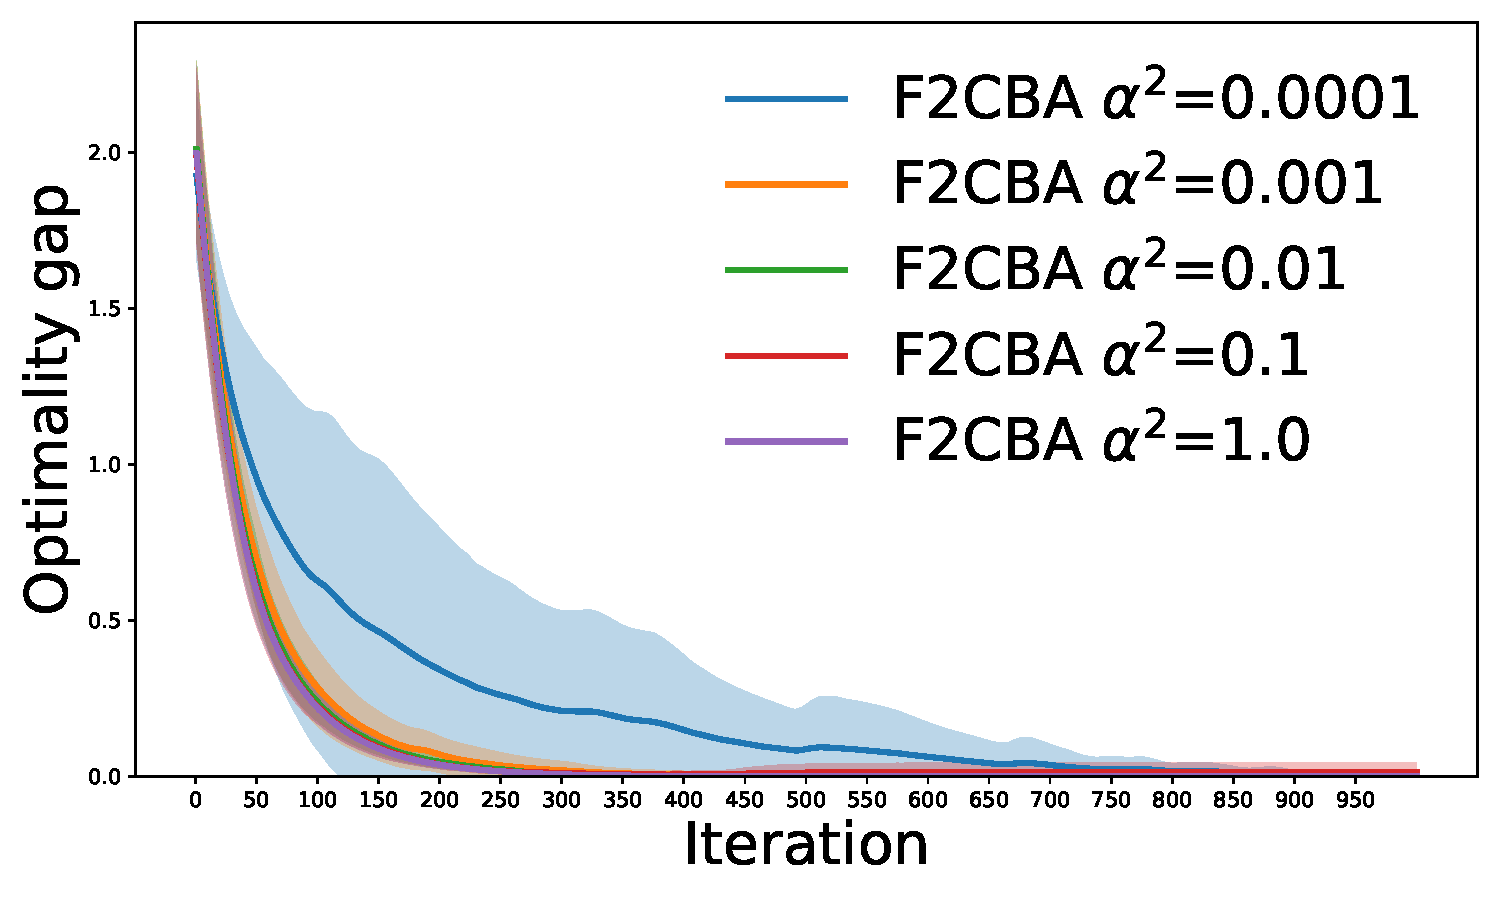
\includegraphics[width=\textwidth]{src/figures/ydim200_gradient_error.pdf}
        \caption{Convergence analysis with varying gradient inexactness $\alpha$.}
        \label{fig:convergence-comparison-2}
    \end{subfigure}
    \hfill
    \begin{subfigure}[b]{0.32\textwidth}
        \centering
        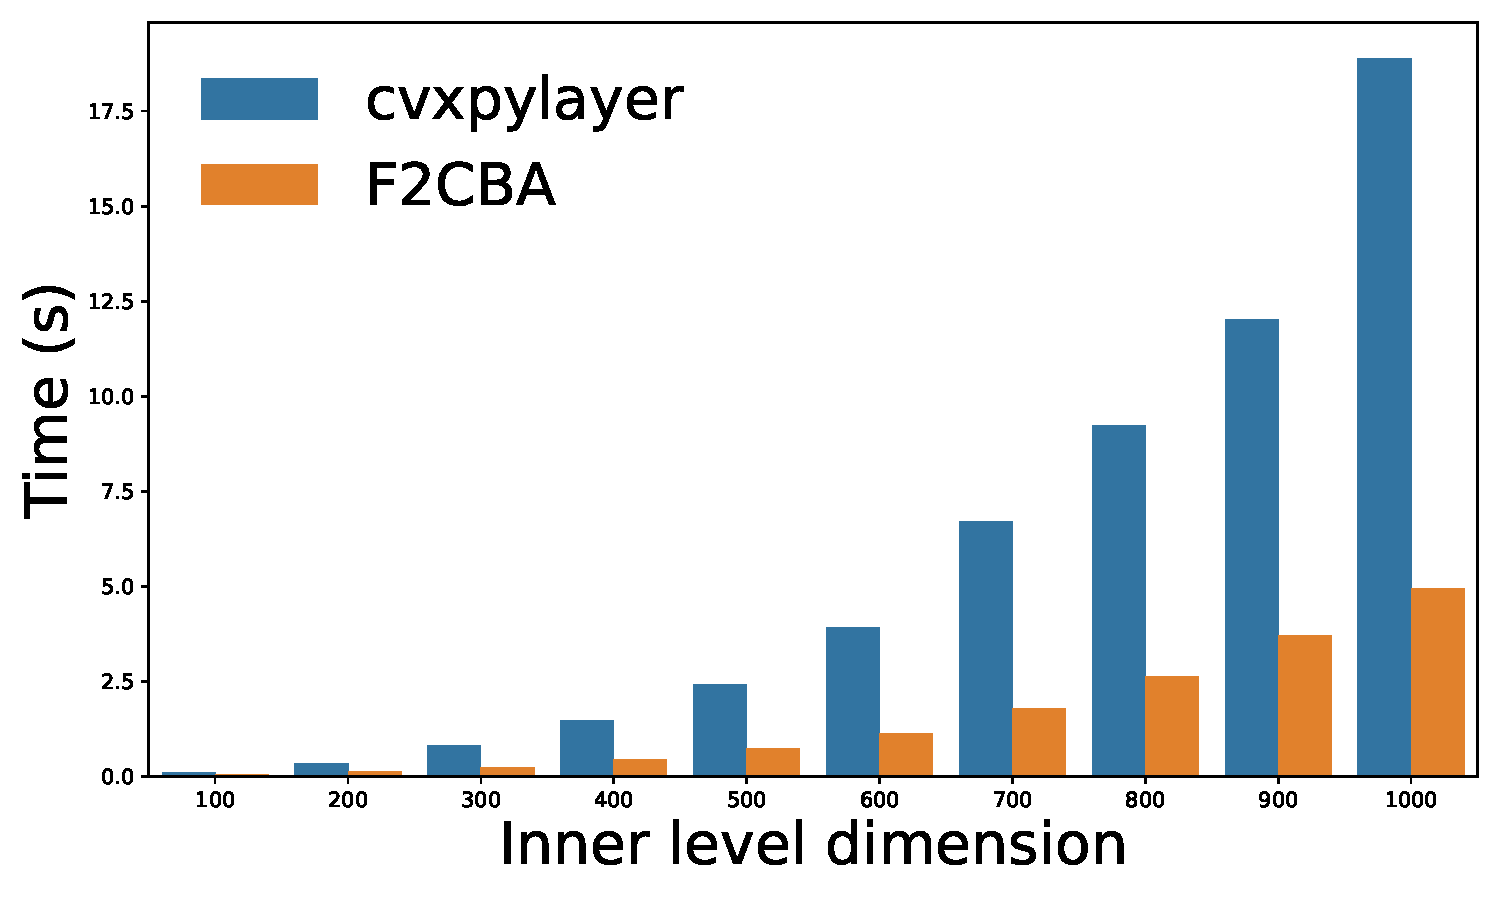
\includegraphics[width=\textwidth]{src/figures/time_results.pdf}
        \caption{Computation cost per gradient step of varying problem size $d_y$.}
        \label{fig:computation-comparison}
    \end{subfigure}
    \caption{We run \cref{alg: PIGD} using \cref{alg:inexact-gradient-oracle} on the bilevel optimization in the toy example in \cref{eqn:experiment-bilevel-optimization} with $d_x = 100$, $d_y = 200$, $n_{\text{const}} = d_y / 5$, and accuracy $\alpha = 1$. \cref{fig:convergence-comparison}, \cref{fig:convergence-comparison-2}, \cref{fig:computation-comparison} vary \# of iterations, gradient exactness $\alpha$, and $d_y$, respectively, to compare the performance under different settings.}
    % Figure~\ref{fig:convergence-comparison} shows that \cref{alg: PIGD} converges in the same rate as CvxpyLayer, while the gradient errors at each iteration are plotted in the colorful bars and are mostly below $\alpha = 0.1$ as guaranteed. Figure~\ref{fig:convergence-comparison-2} shows the convergence under different gradient inexactness $\alpha$. Figure~\ref{fig:computation-comparison} shows the computation cost of both methods under different lower level problem size $d_y$.}
    \label{fig:three graphs}
\end{figure}

We randomly generate the following constrained bilevel optimization problems. 
\begin{align*}\numberthis\label[prob]{eqn:experiment-bilevel-optimization}
     & \mbox{minimize}_{x} ~  c^\top y^* + 0.01 \norm{x}^2 + 0.01 \norm{y^*}^2 ~\text{ subject to } ~ y^* = \argmin_{y: h(x,y) \leq 0} \frac{1}{2} y^\top Q y + x^\top P y, 
\end{align*}
% \begin{align}\label{}
%     \min\nolimits_{x} \quad & \\
%     \text{s.t.} \quad & \nonumber
% \end{align}
where $h_i(x,y) = x^\top A_i y - x^\top b_i ~\forall i \in [K]$ are $K$ bilinear constraints. The PSD matrix $Q \in \reals^{d_y \times d_y}$, $c \in \reals^{d_y}$, $P \in \reals^{d_x \times d_y}$, and constraints $A_i \in \reals^{d_x \times d_y}$, $b_i \in \reals^{d_x}$ are randomly generated from normal distributions (cf. \cref{appendix:experiment-setup}).
We compare our \cref{alg: PIGD} with a non-fully first-order method implemented using \texttt{cvxpyLayer}~\cite{agrawal2019differentiable}. Both algorithms use Adam~\cite{kingma2014adam} to control the learning rate in gradient descent. All the experiments are averaged over ten random seeds.

% \paragraph{Convergence and computation comparisons:} 
\looseness=-1\cref{fig:convergence-comparison} shows that  
% compares the convergence of both methods. We can see that 
both the algorithms converge to the same optimal solution, while the fully first-order method is slightly more stable. Simultaneously, the colorful bars represent the gradient difference between two methods, showing the inexactness of gradient.
\cref{fig:convergence-comparison-2} additionally varies the inexactness to demonstrate its impact to convergence. One can find that too accurate gradient may also harm the convergence due to instability from poor condition numbers.
\cref{fig:computation-comparison} compares the computation cost of different lower level problem size $d_y$. Our fully first-order method significantly outperforms the differentiable optimization method in computation cost.